\section{Mission and Foundations}
% ----------------------------------------------------------------------------
% OPENING SECTION: MISSION, SYSTEM VISION, AND LEARNING ROADMAP
% ---------------------------------------- ------------------------------------

\begin{frame}{First, Observe the Destination}
        
    \begin{figure}
        \centering
        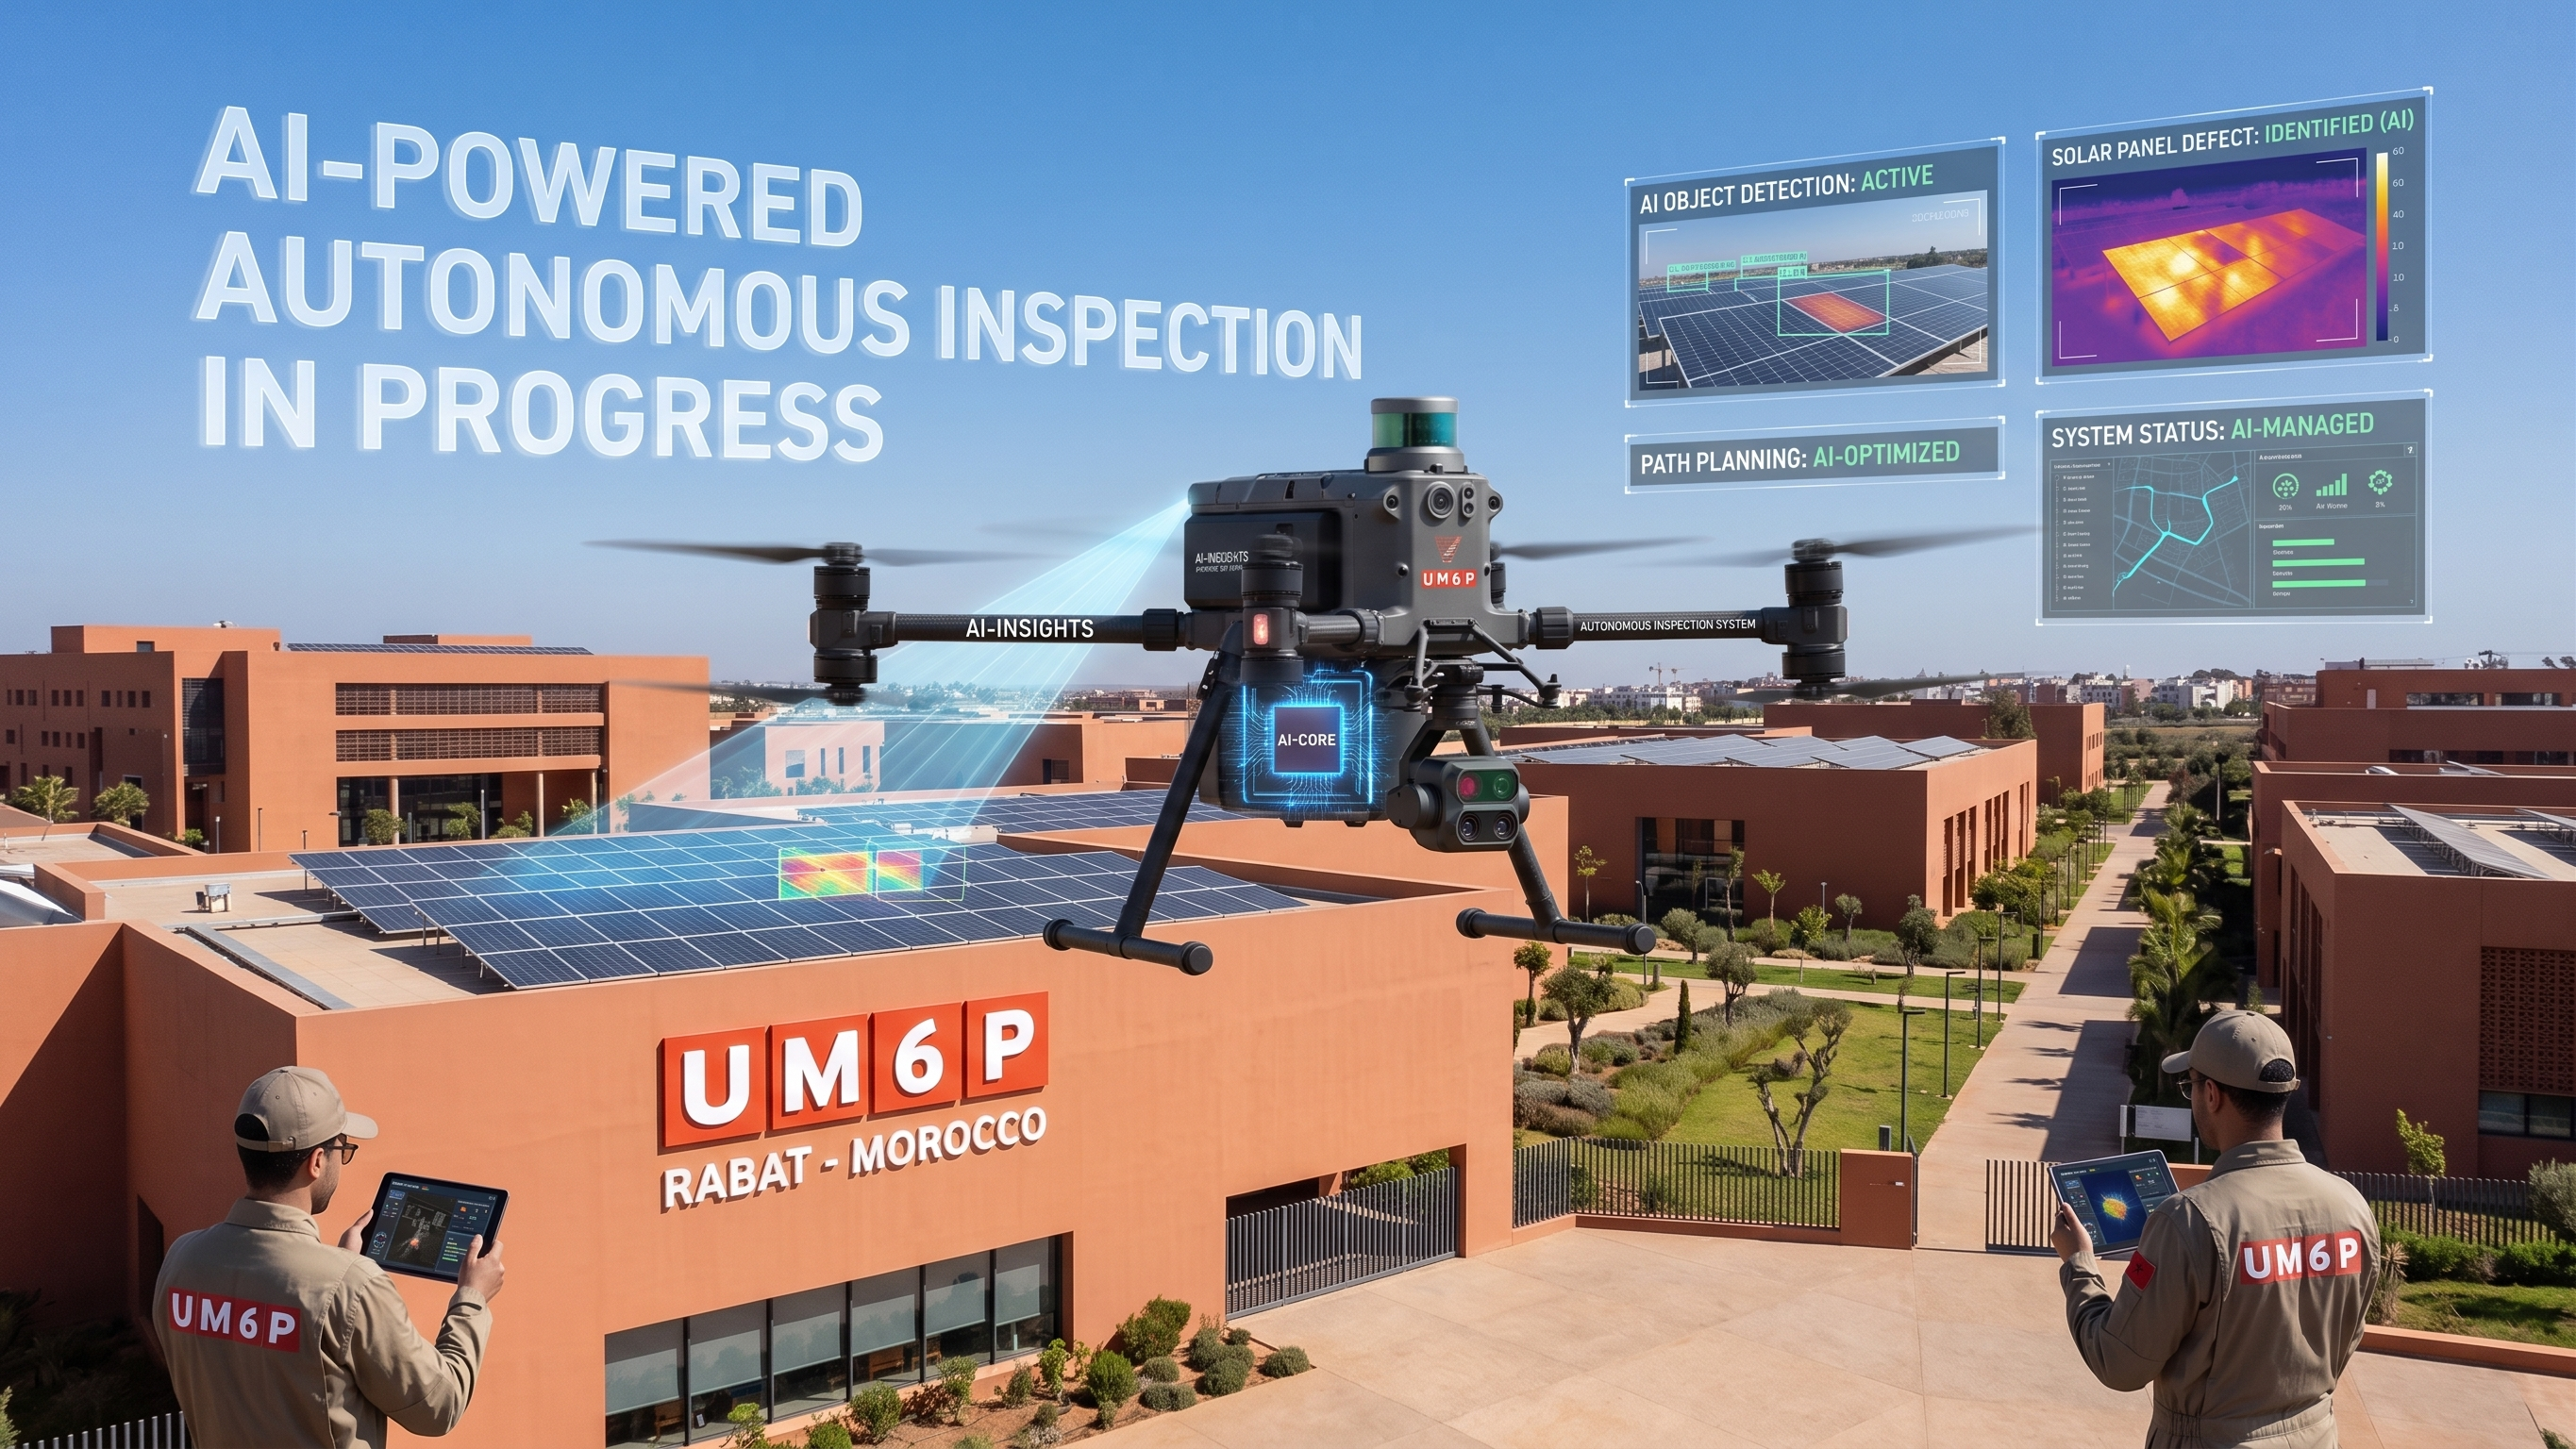
\includegraphics[width=0.9\textwidth]{./images/Gemini_Generated_Image_vo4vdvvo4vdvvo4v.jpeg}
    \end{figure}

\end{frame}

\begin{frame}{The Internship Mission}
\framesubtitle{Build a reproducible autonomous-drone inspection system in simulation}
\footnotesize
\begin{columns}[T,onlytextwidth]
    \begin{column}{0.48\textwidth}
        \begin{block}{Engineering Need}
            Inspection tasks may involve large, repetitive, difficult-to-access,
            or potentially hazardous areas. Aerial robots can help collect
            visual evidence efficiently and consistently.
        \end{block}
    \end{column}
    \pause
    \begin{column}{0.48\textwidth}
        \begin{exampleblock}{Internship Mission}
            Configure, program, simulate, test, and document a quadcopter that:
            \begin{itemize}
                \setlength{\itemsep}{0.22em}
                \item follows a planned inspection mission;
                \item observes a simulated scene with a camera;
                \item detects selected objects;
                \item records useful mission evidence.
            \end{itemize}
        \end{exampleblock}
    \end{column}
\end{columns}
\end{frame}

% ----------------------------------------------------------------------------
\begin{frame}{First, Observe the Destination}

    \footnotesize
\begin{center}
    \Large\bfseries
    Observe the complete demonstration before studying its components.
\end{center}
\vspace{0.35cm}
\begin{center}
\footnotesize
Gazebo world
$\longrightarrow$
PX4-controlled flight
$\longrightarrow$
ROS 2 data exchange
$\longrightarrow$
Camera perception
$\longrightarrow$
Mission evidence
\end{center}

\begin{alertblock}{Important Boundary}
A successful simulation is evidence of software integration, not proof that a real aircraft is ready or safe to fly.
\end{alertblock}

\end{frame}


\begin{frame}{First, Observe the Destination}
        
    \begin{figure}
        \centering
        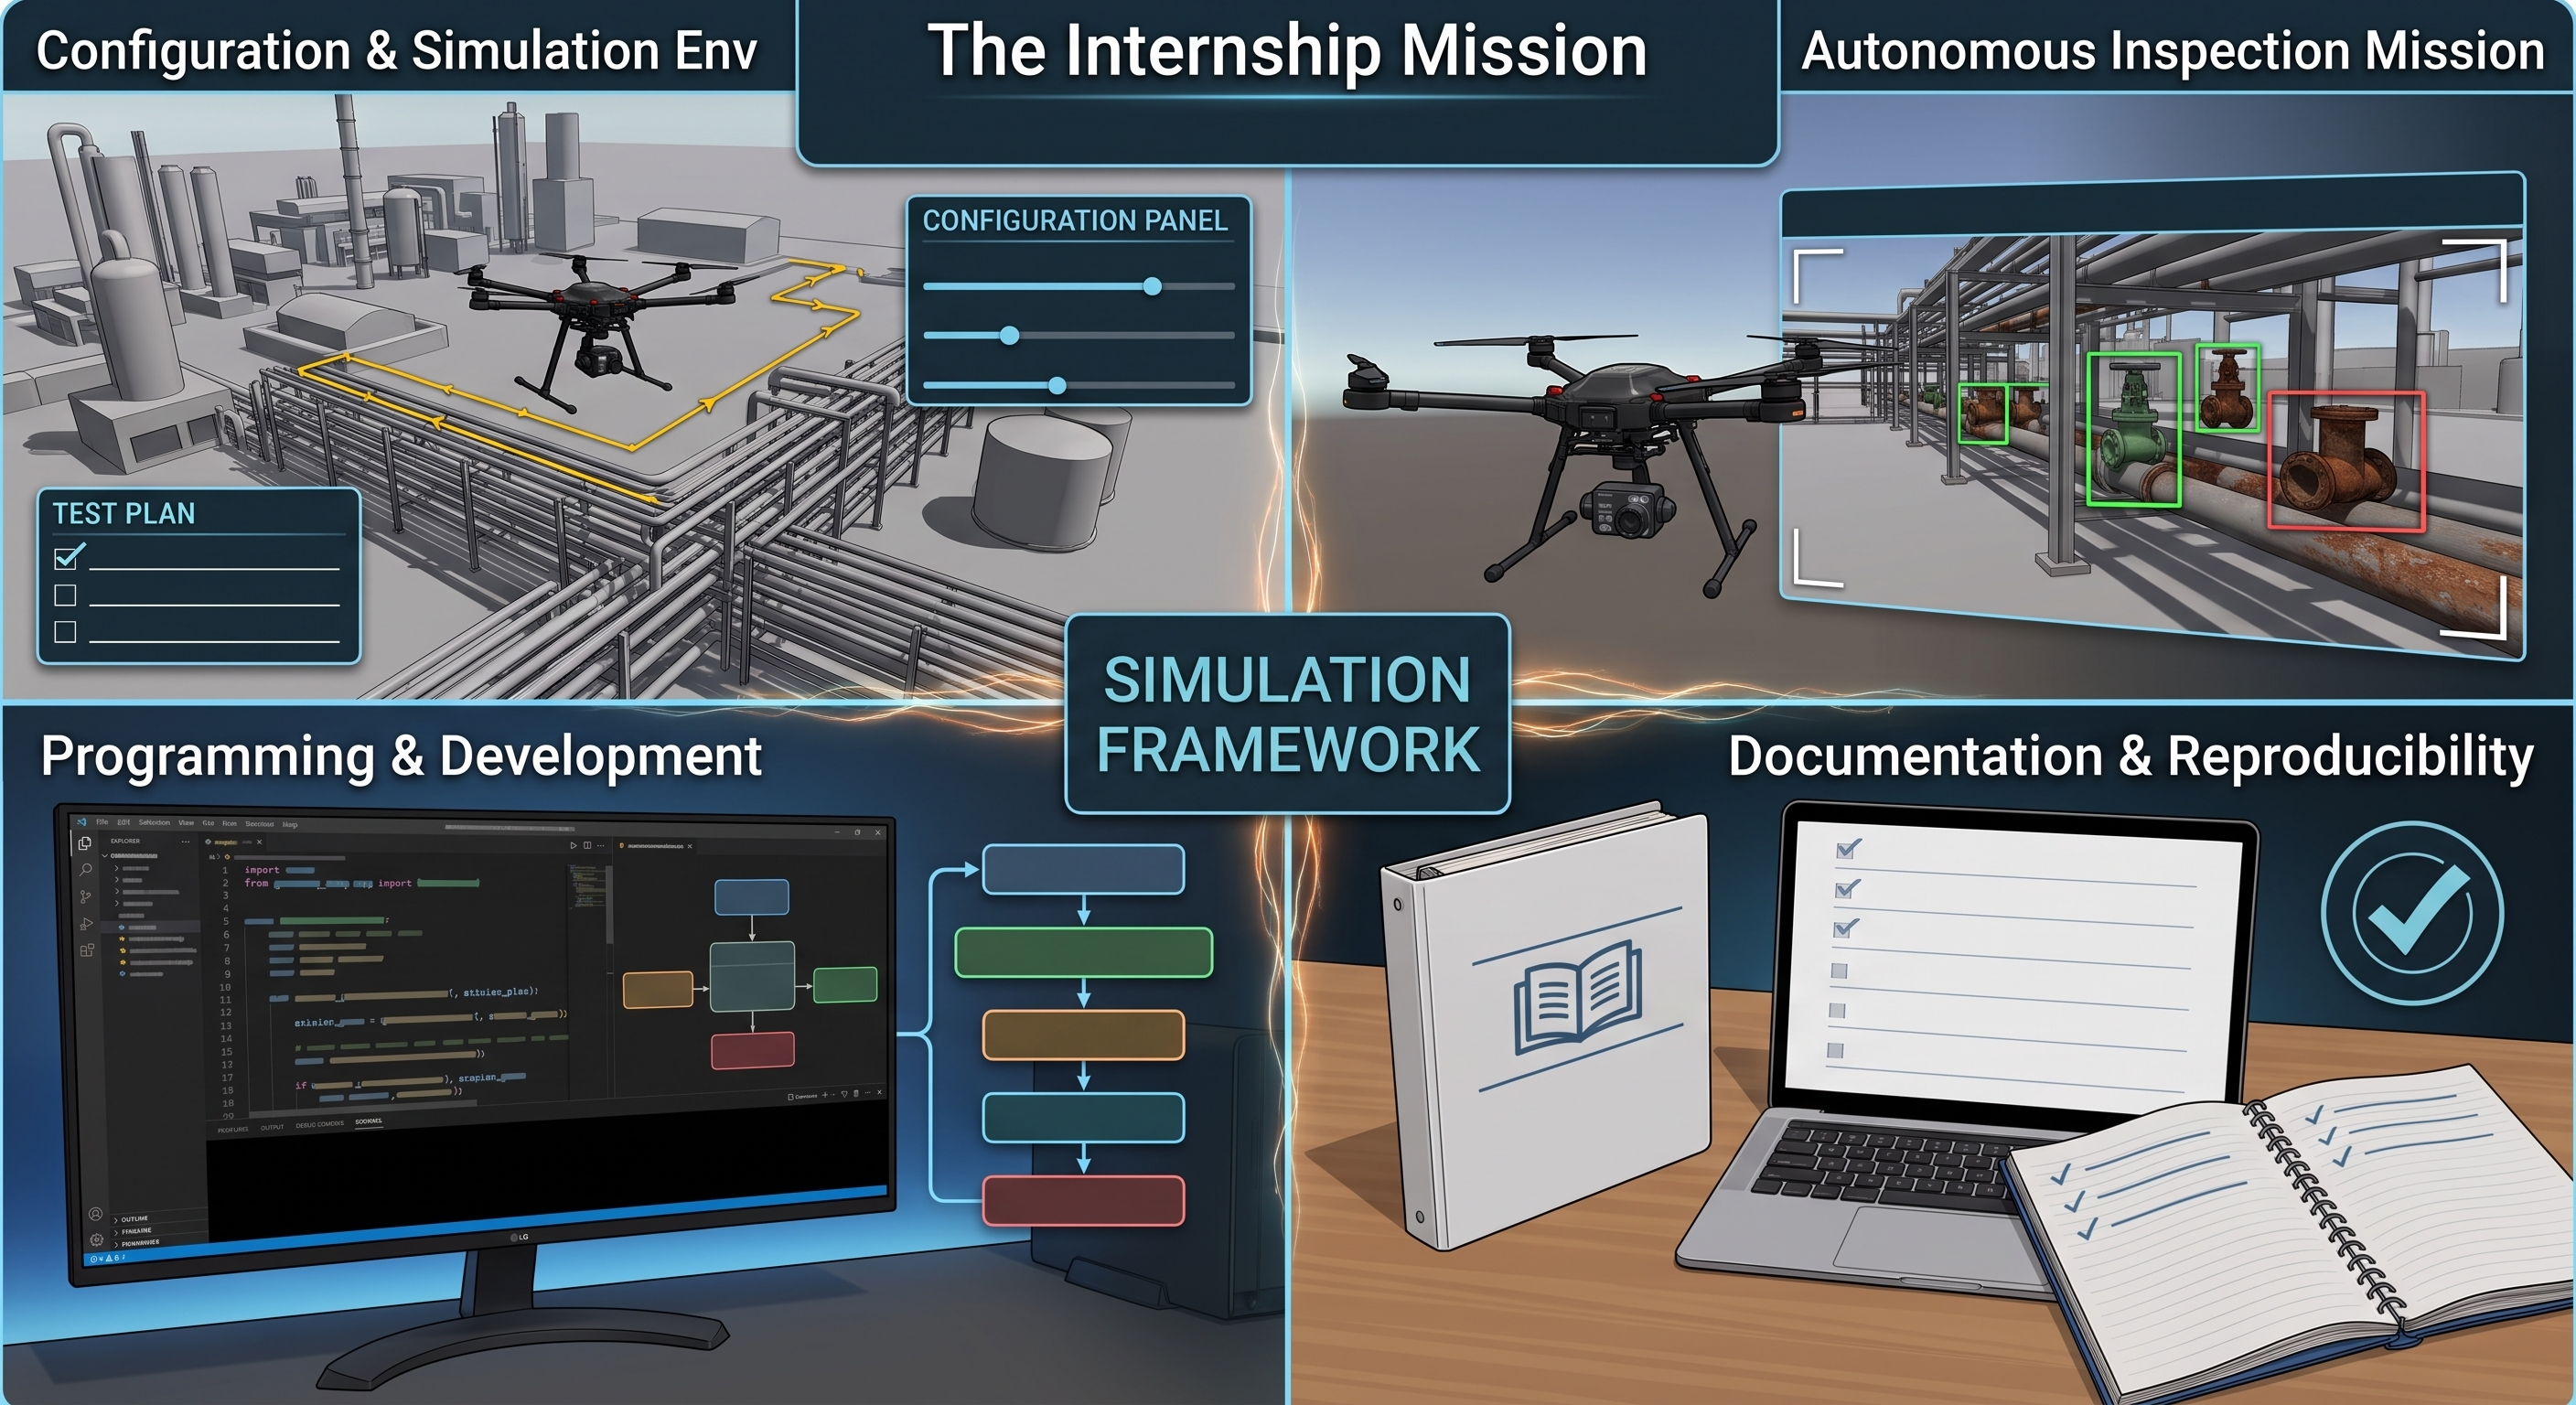
\includegraphics[width=0.9\textwidth]{./images/intershipimg.jpeg}
    \end{figure}

\end{frame}



% % ----------------------------------------------------------------------------
% \begin{frame}{The Expected Final Demonstration}
% \framesubtitle{What the completed GitHub-based project should reproduce}
% \footnotesize
% \begin{columns}[T,onlytextwidth]
%     \begin{column}{0.32\textwidth}
%         \begin{block}{1. Launch}
%             Start the required simulation, flight-control, communication, and perception processes from a documented workspace.
%         \end{block}
%     \end{column}
%     \pause
%     \begin{column}{0.32\textwidth}
%         \begin{block}{2. Observe}
%             Watch the vehicle, mission state, camera stream, ROS 2 interfaces, and detector outputs.
%         \end{block}
%     \end{column}
%     \pause
%     \begin{column}{0.32\textwidth}
%         \begin{block}{3. Verify}
%             Compare intended behavior with logs, messages, detections, screenshots, and saved mission evidence.
%         \end{block}
%     \end{column}
% \end{columns}
% \begin{exampleblock}{Definition of Success}
% The system launches predictably, its components exchange the expected information, the simulated drone executes the intended mission, and the results can be explained and reproduced from the repository documentation.
% \end{exampleblock}
% \end{frame}

% ----------------------------------------------------------------------------
\begin{frame}{The Engineering Challenge}
\framesubtitle{One visible mission depends on several connected technical layers}
\footnotesize
\begin{block}{Why Is the Project Technically Interesting?}
A drone inspection mission is a \textbf{system-of-systems problem}. Motion, sensing, communication, software, perception, testing, and documentation must work together.
\end{block}
\begin{center}
% \scriptsize
\textbf{
Operating environment
$\rightarrow$
Simulation
$\rightarrow$
Flight control
$\rightarrow$
Communication
$\rightarrow$
Perception
$\rightarrow$
Evidence
}
\end{center}
\pause
\begin{alertblock}{A Chain Is Verified Link by Link}
A detector cannot process a missing camera stream. A mission node cannot guide the vehicle through an incorrect interface. A working local setup cannot be reproduced without controlled dependencies and documentation.
\end{alertblock}
\end{frame}

% ----------------------------------------------------------------------------
\begin{frame}{The Student Journey}
\framesubtitle{Progress from guided reproduction to engineering ownership}
\footnotesize
\begin{enumerate}
    \setlength{\itemsep}{0.35em}
    \item \textbf{Orient:} understand the mission, architecture, repository, and expected evidence.
    \item \textbf{Prepare:} configure Ubuntu, tools, dependencies, workspace, and project files.
    \item \textbf{Learn the foundations:} practise Bash, Git, Python, ROS 2, Gazebo, PX4, and perception concepts in context.
    \item \textbf{Integrate:} connect mission logic, simulated flight, camera data, and object detection.
    \item \textbf{Verify:} test one layer at a time before testing the complete pipeline.
    \item \textbf{Deliver:} publish reproducible code, configuration, evidence, documentation, and a technical report.
\end{enumerate}
\end{frame}






\begin{frame}{One Project, Several Foundations}
\framesubtitle{A complete robotic system is built layer by layer}

\footnotesize

\begin{center}
    \large
    \textbf{The drone demonstration is the visible result.}\\[0.3em]
    \normalsize
    Behind it, several technical foundations must work together.
\end{center}

\pause

\begin{columns}[T,onlytextwidth]
    \begin{column}{0.30\textwidth}
        \begin{block}{Prepare}
            Configure the computer and create a reproducible project environment.
        \end{block}
    \end{column}
    \hfill
    \begin{column}{0.30\textwidth}
        \begin{block}{Build}
            Program, simulate, connect, and test the robotic components.
        \end{block}
    \end{column}
    \hfill
    \begin{column}{0.30\textwidth}
        \begin{block}{Deliver}
            Document the work, preserve the results, and share a working project.
        \end{block}
    \end{column}
\end{columns}

\pause

\begin{exampleblock}{Think of the Project as a Team}
    Ubuntu provides the workplace, Bash executes instructions, Git preserves progress,
    Python implements logic, ROS~2 connects components, Gazebo provides the simulated
    world, and AI interprets camera data.
\end{exampleblock}

\begin{center}
    \textbf{You are not expected to master everything on Day~1.}\\
    You will learn each foundation when the project needs it.
\end{center}
\end{frame}


\begin{frame}{Technology Ecosystem I}
\framesubtitle{Preparing the environment and preserving your work}

\footnotesize

\begin{columns}[T,onlytextwidth]
    \begin{column}{0.48\textwidth}
        \begin{block}{Ubuntu: The Workplace}
            Ubuntu is the Linux distribution used to run the project.
            It provides the files, processes, packages, and services
            required by the robotics tools.
        \end{block}

        \begin{block}{Terminal and Bash: The Control Desk}
            The \textbf{terminal} is the window where commands are entered.
            \textbf{Bash} is the shell that reads and executes those commands,
            variables, and scripts.
        \end{block}
    \end{column}
    \hfill
    \begin{column}{0.48\textwidth}
        \begin{block}{Git: The Project Timeline}
            Git records changes on the computer. It allows students to create
            checkpoints, compare versions, and recover a previous working state.
        \end{block}

        \begin{block}{GitHub: The Shared Project Home}
            GitHub hosts the Git repository online. It supports collaboration,
            documentation, issue tracking, review, and delivery of the internship
            project.
        \end{block}
    \end{column}
\end{columns}

\pause

\begin{exampleblock}{How These Foundations Support the Drone Project}
    \centering
    \textbf{Ubuntu} runs the tools
    \(\rightarrow\)
    \textbf{Bash} launches the workflow
    \(\rightarrow\)
    \textbf{Git} preserves the work
    \(\rightarrow\)
    \textbf{GitHub} makes the project reproducible and shareable.
\end{exampleblock}
\end{frame}



































% ----------------------------------------------------------------------------
\begin{frame}{Technology Ecosystem I}
\framesubtitle{The engineering environment and reproducible workflow}
\footnotesize
\begin{columns}[T,onlytextwidth]
    \begin{column}{0.48\textwidth}
        \begin{block}{Ubuntu and Linux}
            \textbf{Ubuntu} is the Linux distribution used as the project environment. It provides the filesystem, processes, users, packages, and services on which the robotics tools run.
        \end{block}
        \begin{block}{Terminal and Bash}
            The \textbf{terminal} is the text-based interface window. \textbf{Bash} is the shell that interprets commands, variables, scripts, and environment configuration entered through it.
        \end{block}
    \end{column}
    \begin{column}{0.48\textwidth}
        \begin{block}{Git}
            Git records project history locally. Students use it to inspect changes, create commits, recover earlier states, and work systematically.
        \end{block}
        \begin{block}{GitHub}
            GitHub hosts and shares the Git repository. It supports collaboration, documentation, issue tracking, review, and delivery of the reproducible internship project.
        \end{block}
    \end{column}
\end{columns}

\pause
\begin{exampleblock}{Project Connection}
These foundations help you install the environment, obtain the repository, run documented commands, diagnose problems, preserve changes, and share verified results.
\end{exampleblock}
\end{frame}

% ----------------------------------------------------------------------------
\begin{frame}{Technology Ecosystem II}
\framesubtitle{Programming, integration, simulation, control, and perception}
\scriptsize
\renewcommand{\arraystretch}{1.18}
\begin{tabularx}{\textwidth}{>{\bfseries\color{um6p-color-dark-blue}}p{0.15\textwidth} X X}
\toprule
Technology & Intuitive Role & Internship Use \\
\midrule
Python & Practical programming language for readable robotics logic and data processing & ROS 2 nodes, mission utilities, image handling, AI integration, and tests \\
ROS 2 & Communication and integration framework, not an operating system & Connect nodes through typed topics, messages, services, parameters, and packages \\
Gazebo & Simulated world containing the drone, sensors, objects, environment, and physics & Develop and observe the mission without claiming real-world flight readiness \\
PX4 & Autopilot responsible for estimation, stabilization, and tracking flight references & Convert mission references into controlled simulated vehicle motion \\
AI / YOLOv8 & Perception component that transforms camera images into object detections & Produce observations for mission evidence; it does not directly guarantee safe control \\
\bottomrule
\end{tabularx}
\begin{alertblock}{Responsibility Boundary}
Object detection answers, ``What may be visible in this image?'' Autonomous control answers, ``How should the vehicle move safely?'' These are connected responsibilities, not the same function.
\end{alertblock}
\end{frame}

% ----------------------------------------------------------------------------
\begin{frame}{Complete System Pipeline}
\framesubtitle{From engineering environment to reproducible mission evidence}
\footnotesize
\begin{block}{Foundation and Execution Layer}
\centering
Ubuntu $+$ Terminal/Bash $+$ Python environment
$\longrightarrow$
workspace, dependencies, scripts, and running processes
\end{block}
\pause
\begin{block}{Command Flow: Mission Decision to Simulated Motion}
\centering
ROS 2 mission node
$\longrightarrow$
Micro XRCE-DDS
$\longrightarrow$
PX4 autopilot
$\longrightarrow$
Gazebo drone physics
\end{block}
\pause
\begin{exampleblock}{Evidence Flow: Simulated World to Inspection Result}
\centering
Simulated camera
$\longrightarrow$
ROS-Gazebo image bridge
$\longrightarrow$
YOLOv8 detector
$\longrightarrow$
mission evidence and report
\end{exampleblock}
\pause
\begin{alertblock}{Reproducibility Layer}
Git and GitHub preserve the source code, configuration, history, instructions, tests, limitations, and evidence required to rebuild the complete pipeline.
\end{alertblock}
\end{frame}

% ----------------------------------------------------------------------------
\begin{frame}{How We Will Study Each Foundation}
\framesubtitle{A repeated reasoning pattern for every tutorial}
\footnotesize
\begin{enumerate}
    \setlength{\itemsep}{0.35em}
    \item \textbf{Why?} Which project problem does this foundation solve?
    \item \textbf{What?} What does it mean at an intuitive and technically correct level?
    \item \textbf{How does it fit?} Where is it located in the complete pipeline?
    \item \textbf{Project connection?} Which file, process, command, node, topic, or result uses it?
    \item \textbf{Verification?} What observable output confirms correct behavior?
    \item \textbf{Next step?} Which later tutorial develops the idea in greater depth?
\end{enumerate}
\begin{exampleblock}{Example}
Before studying ROS 2 details, students first recognize its system role: it carries typed information between software components and makes their interfaces observable and testable.
\end{exampleblock}
\end{frame}

% ----------------------------------------------------------------------------
\begin{frame}{Professional Working Method}
\framesubtitle{Progress is created through disciplined observation}
\footnotesize
\begin{columns}[T,onlytextwidth]
    \begin{column}{0.48\textwidth}
        \begin{block}{Before Execution}
            \begin{itemize}
                \setlength{\itemsep}{0.22em}
                \item identify the current directory and environment;
                \item predict the expected output;
                \item understand which component will be affected;
                \item change one factor at a time.
            \end{itemize}
        \end{block}
    \end{column}
    \begin{column}{0.48\textwidth}
        \begin{block}{After Execution}
            \begin{itemize}
                \setlength{\itemsep}{0.22em}
                \item read complete outputs and error messages;
                \item compare observation with expectation;
                \item preserve commands, logs, and screenshots;
                \item document results and limitations honestly.
            \end{itemize}
        \end{block}
    \end{column}
\end{columns}
\begin{alertblock}{Engineering Habit}
A desired trajectory, a clean visualization, or a single successful launch is not sufficient evidence. Each important claim must be supported by an observable test.
\end{alertblock}
\end{frame}

% ----------------------------------------------------------------------------
\begin{frame}{Internship Deliverables}
\framesubtitle{What students are expected to build and submit}
\footnotesize
\begin{columns}[T,onlytextwidth]
    \begin{column}{0.48\textwidth}
        \begin{block}{Working Engineering Assets}
            \begin{itemize}
                \setlength{\itemsep}{0.22em}
                \item structured Git repository and clear history;
                \item reproducible environment and configuration;
                \item ROS 2 packages, Python source code, and launch files;
                \item working Gazebo/PX4 inspection simulation;
                \item camera and object-detection integration.
            \end{itemize}
        \end{block}
    \end{column}
    \begin{column}{0.48\textwidth}
        \begin{exampleblock}{Evidence and Communication}
            \begin{itemize}
                \setlength{\itemsep}{0.22em}
                \item layer-level and end-to-end tests;
                \item logs, screenshots, and mission results;
                \item installation and execution instructions;
                \item final demonstration;
                \item technical report with results, limitations, and future work.
            \end{itemize}
        \end{exampleblock}
    \end{column}
\end{columns}
\begin{alertblock}{Delivery Standard}
A reviewer should be able to clone the repository, follow the documentation, reproduce the demonstration, and understand what was verified.
\end{alertblock}
\end{frame}

% ----------------------------------------------------------------------------
\begin{frame}{Knowledge Check}
\framesubtitle{Can you explain the project before implementing it?}
\footnotesize
\begin{columns}[T,onlytextwidth]
    \begin{column}{0.48\textwidth}
        \begin{block}{Mission and Architecture}
            \begin{enumerate}
                \setlength{\itemsep}{0.2em}
                \item What useful inspection outcome should the system produce?
                \item Why is this a systems-engineering project?
                \item Which components simulate physics, stabilize flight, and exchange information?
            \end{enumerate}
        \end{block}
    \end{column}
    \begin{column}{0.48\textwidth}
        \begin{block}{Verification and Boundaries}
            \begin{enumerate}
                \setlength{\itemsep}{0.2em}
                \item Why verify the camera stream before the detector?
                \item Why is detection different from control?
                \item Why does simulation success not prove real-flight readiness?
            \end{enumerate}
        \end{block}
    \end{column}
\end{columns}
\begin{exampleblock}{Expected Explanation}
Describe the mission, command flow, evidence flow, role of each major technology, and the evidence required to reproduce the result.
\end{exampleblock}
\end{frame}

% ----------------------------------------------------------------------------
\begin{frame}{Learning Roadmap}
\framesubtitle{Each foundation unlocks one part of the final GitHub project}
\scriptsize
\renewcommand{\arraystretch}{1.16}
\begin{tabularx}{\textwidth}{>{\bfseries\color{um6p-color-dark-blue}}p{0.22\textwidth} X >{\centering\arraybackslash}p{0.24\textwidth}}
\toprule
Foundation & Contribution to the Project & Practical Outcome \\
\midrule
Ubuntu & Provides the Linux engineering environment & Prepare the workstation \\
Terminal and Bash & Operate, configure, launch, inspect, and troubleshoot & Run the documented workflow \\
Git and GitHub & Preserve and share a reproducible project & Clone, manage, document, and deliver \\
Python for robotics & Express logic and process project data & Read and modify project programs \\
ROS 2 & Connect software components through defined interfaces & Build and verify communication \\
Gazebo and PX4 & Simulate the world and controlled drone motion & Execute the inspection mission \\
AI integration & Convert camera data into perception results & Produce inspection evidence \\
\bottomrule
\end{tabularx}
\begin{alertblock}{End-to-End Objective}
The tutorials are not isolated courses. Together, they provide the foundations required to reproduce, understand, test, and improve the autonomous-drone project hosted on GitHub.
\end{alertblock}
\end{frame}

% ----------------------------------------------------------------------------
\begin{frame}{Transition to the Technical Foundations}
\framesubtitle{Build the environment before building the autonomous system}
\begin{center}
{\Large\bfseries\color{um6p-dark}
Next: Ubuntu and the Linux Engineering Environment}
\end{center}
\vspace{0.35cm}
\begin{center}
\footnotesize
Ubuntu
$\rightarrow$
Terminal and Bash
$\rightarrow$
Git and GitHub
$\rightarrow$
Python
$\rightarrow$
ROS 2
$\rightarrow$ 
Gazebo and PX4
$\rightarrow$
AI integration
\end{center}
\begin{exampleblock}{Guiding Question}
What must be installed, organized, and verified so that every later component can run reliably inside the same engineering environment?
\end{exampleblock}
\end{frame}
   